\documentclass[tikz,border=12pt]{standalone}
\usepackage[T1]{fontenc}
\usepackage{tgheros}
\usepackage{sfmath}
\usepackage{amsmath}
\usepackage{amssymb}
\usepackage{tikz}
\usetikzlibrary{arrows.meta,positioning,shapes.geometric,fit,backgrounds,calc}
\usepackage{xcolor}

\renewcommand{\familydefault}{\sfdefault}

% Harvard Crimson & ETH Zurich Academic Semantic Palette
\definecolor{harvardcrimson}{HTML}{A51C30}
\definecolor{ethdarkblue}{HTML}{1F407A}
\definecolor{ethblue}{HTML}{215CAF}
\definecolor{ethpetrol}{HTML}{007A87}
\definecolor{ethbronze}{HTML}{B87333}
\definecolor{ethslate}{HTML}{475569}
\definecolor{cardbg}{HTML}{F8FAFC}
\definecolor{cardborder}{HTML}{CBD5E1}
\definecolor{lightpetrol}{HTML}{E6F4F6}
\definecolor{lightbronze}{HTML}{FAF0E6}
\definecolor{lightcrimson}{HTML}{FDF2F4}
\definecolor{lightnavy}{HTML}{EDF2F9}

\begin{document}
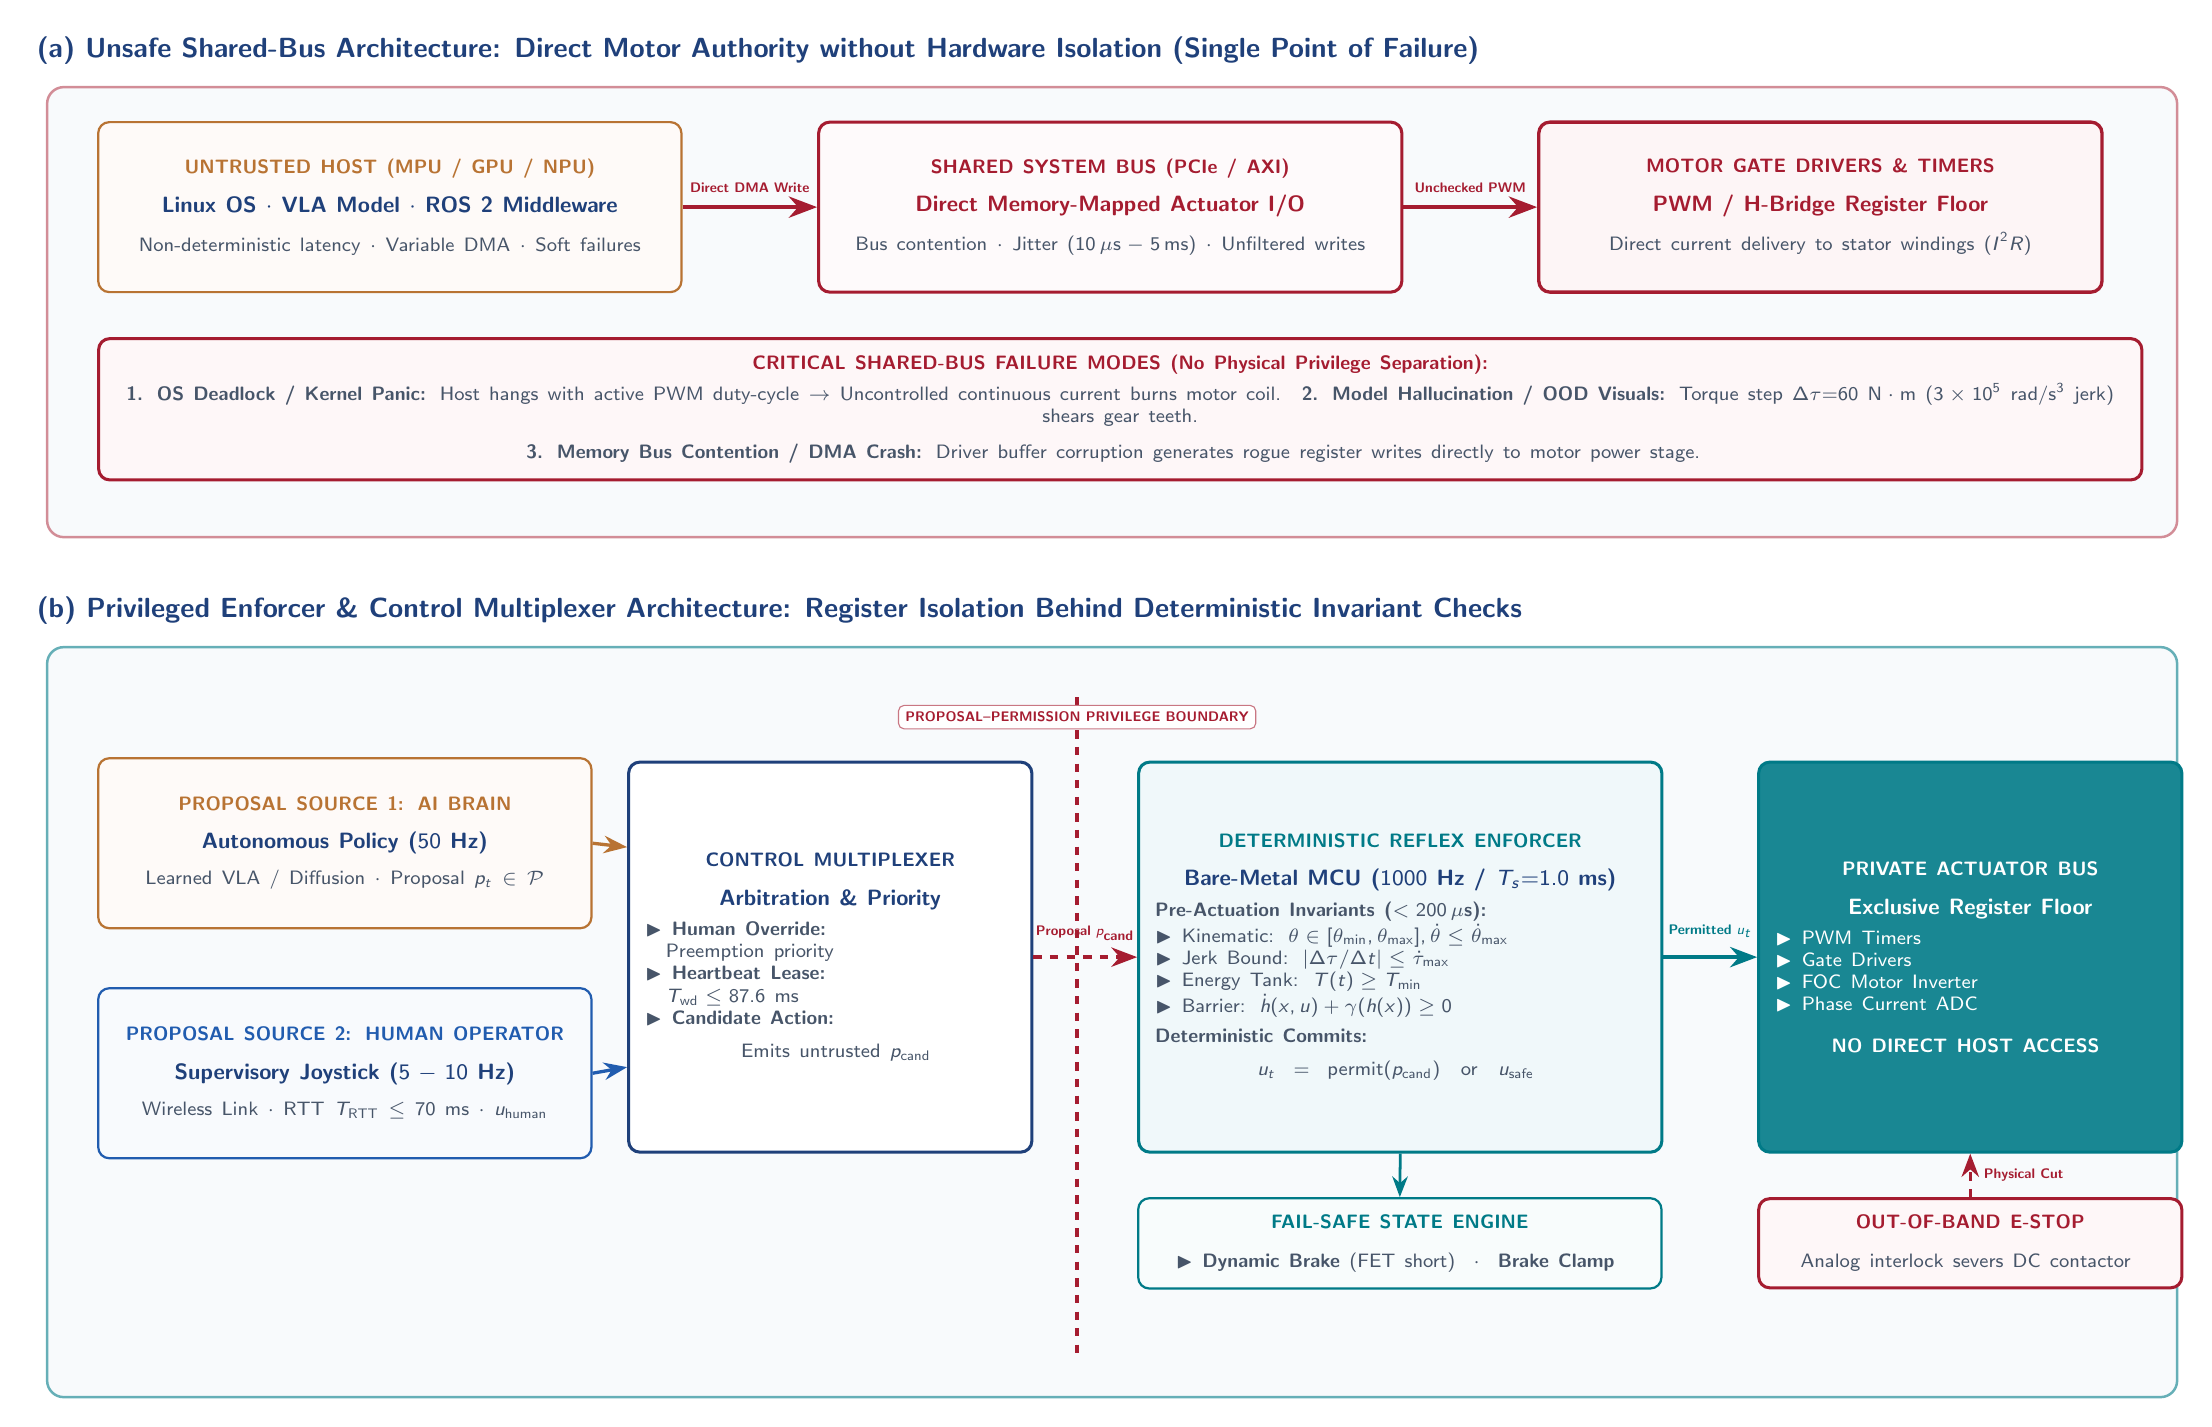
\begin{tikzpicture}[
  font=\sffamily,
  >=Stealth,
  sectionbox/.style={
    draw=cardborder,
    fill=cardbg,
    rounded corners=6pt,
    line width=0.9pt,
    inner sep=10pt
  },
  card/.style={
    draw=cardborder,
    fill=white,
    rounded corners=4pt,
    line width=0.8pt,
    inner sep=6pt,
    align=center
  },
  alertcard/.style={
    draw=harvardcrimson,
    fill=lightcrimson!60,
    rounded corners=4pt,
    line width=1.1pt,
    inner sep=6pt,
    align=center
  },
  safecard/.style={
    draw=ethpetrol,
    fill=lightpetrol!60,
    rounded corners=4pt,
    line width=1.1pt,
    inner sep=6pt,
    align=center
  }
]

  % =========================================================================
  % TOP PANEL: UNSAFE SHARED-BUS ARCHITECTURE (ANTI-PATTERN)
  % =========================================================================

  \node[font=\sffamily\bfseries\normalsize, text=ethdarkblue, anchor=north west] (top_title) at (0,0) {
    (a) Unsafe Shared-Bus Architecture: Direct Motor Authority without Hardware Isolation (Single Point of Failure)
  };

  % Unsafe Container Box
  \draw[draw=harvardcrimson!50, fill=cardbg, rounded corners=6pt, line width=0.9pt] (0.10in, -0.30in) rectangle (10.75in, -2.55in);

  % Unsafe Host Block (Linux MPU + Model)
  \node[card, draw=ethbronze, fill=lightbronze!30, text width=2.75in, minimum height=0.85in, anchor=west] (unsafe_mpu) at (0.35in, -0.90in) {
    {\scriptsize\bfseries\color{ethbronze}UNTRUSTED HOST (MPU / GPU / NPU)}\\[2pt]
    {\footnotesize\bfseries\color{ethdarkblue}Linux OS $\cdot$ VLA Model $\cdot$ ROS 2 Middleware}\\[2pt]
    {\scriptsize\color{ethslate}Non-deterministic latency $\cdot$ Variable DMA $\cdot$ Soft failures}
  };

  % Shared System Bus
  \node[card, draw=harvardcrimson, fill=lightcrimson!40, line width=1.1pt, text width=2.75in, minimum height=0.85in, anchor=west] (shared_bus) at (3.95in, -0.90in) {
    {\scriptsize\bfseries\color{harvardcrimson}SHARED SYSTEM BUS (PCIe / AXI)}\\[2pt]
    {\footnotesize\bfseries\color{harvardcrimson}Direct Memory-Mapped Actuator I/O}\\[2pt]
    {\scriptsize\color{ethslate}Bus contention $\cdot$ Jitter ($10\,\mu\text{s}-5\,\text{ms}$) $\cdot$ Unfiltered writes}
  };

  % Motor Drive Register Floor
  \node[card, draw=harvardcrimson, fill=lightcrimson!80, line width=1.2pt, text width=2.65in, minimum height=0.85in, anchor=west] (unsafe_registers) at (7.55in, -0.90in) {
    {\scriptsize\bfseries\color{harvardcrimson}MOTOR GATE DRIVERS \& TIMERS}\\[2pt]
    {\footnotesize\bfseries\color{harvardcrimson}PWM / H-Bridge Register Floor}\\[2pt]
    {\scriptsize\color{ethslate}Direct current delivery to stator windings ($I^2R$)}
  };

  % Direct Unsafe Path Arrows
  \draw[->, line width=1.6pt, harvardcrimson] (unsafe_mpu.east) -- node[above=1pt, font=\sffamily\bfseries\tiny, text=harvardcrimson]{Direct DMA Write} (shared_bus.west);
  \draw[->, line width=1.6pt, harvardcrimson] (shared_bus.east) -- node[above=1pt, font=\sffamily\bfseries\tiny, text=harvardcrimson]{Unchecked PWM} (unsafe_registers.west);

  % Failure Mode Annotations below
  \node[alertcard, text width=10.05in, anchor=north west] (unsafe_faults) at (0.35in, -1.55in) {
    {\scriptsize\bfseries\color{harvardcrimson}CRITICAL SHARED-BUS FAILURE MODES (No Physical Privilege Separation):}\\[2pt]
    {\scriptsize\color{ethslate}
    \textbf{1. OS Deadlock / Kernel Panic:} Host hangs with active PWM duty-cycle $\to$ Uncontrolled continuous current burns motor coil.\quad
    \textbf{2. Model Hallucination / OOD Visuals:} Torque step $\Delta \tau{=}60\text{ N}\cdot\text{m}$ ($3\times 10^5\text{ rad/s}^3$ jerk) shears gear teeth.\\[1pt]
    \textbf{3. Memory Bus Contention / DMA Crash:} Driver buffer corruption generates rogue register writes directly to motor power stage.
    }
  };

  % =========================================================================
  % BOTTOM PANEL: HARDENED DUAL-DOMAIN PRIVILEGED ARCHITECTURE
  % =========================================================================

  \node[font=\sffamily\bfseries\normalsize, text=ethdarkblue, anchor=north west] (bottom_title) at (0, -2.80in) {
    (b) Privileged Enforcer \& Control Multiplexer Architecture: Register Isolation Behind Deterministic Invariant Checks
  };

  % Bottom Container Box
  \draw[draw=ethpetrol!60, fill=cardbg, rounded corners=6pt, line width=0.9pt] (0.10in, -3.10in) rectangle (10.75in, -6.85in);

  % Proposal Tier: Source 1 (Autonomous Brain)
  \node[card, draw=ethbronze, fill=lightbronze!30, text width=2.30in, minimum height=0.85in, anchor=north west] (prop_brain) at (0.35in, -3.65in) {
    {\scriptsize\bfseries\color{ethbronze}PROPOSAL SOURCE 1: AI BRAIN}\\[2pt]
    {\footnotesize\bfseries\color{ethdarkblue}Autonomous Policy ($50\text{ Hz}$)}\\[1pt]
    {\scriptsize\color{ethslate}Learned VLA / Diffusion $\cdot$ Proposal $p_t \in \mathcal{P}$}
  };

  % Proposal Tier: Source 2 (Human Operator)
  \node[card, draw=ethblue, fill=lightnavy!40, text width=2.30in, minimum height=0.85in, anchor=north west] (prop_human) at (0.35in, -4.80in) {
    {\scriptsize\bfseries\color{ethblue}PROPOSAL SOURCE 2: HUMAN OPERATOR}\\[2pt]
    {\footnotesize\bfseries\color{ethdarkblue}Supervisory Joystick ($5-10\text{ Hz}$)}\\[1pt]
    {\scriptsize\color{ethslate}Wireless Link $\cdot$ RTT $T_{\text{RTT}} \le 70\text{ ms}$ $\cdot$ $u_{\text{human}}$}
  };

  % Control Multiplexer Node (centered vertically at y = -4.65in)
  \node[card, draw=ethdarkblue, fill=white, line width=1.1pt, text width=1.85in, minimum height=1.95in, anchor=west] (ctrl_mux) at (3.00in, -4.65in) {
    {\scriptsize\bfseries\color{ethdarkblue}CONTROL MULTIPLEXER}\\[2pt]
    {\footnotesize\bfseries\color{ethdarkblue}Arbitration \& Priority}\\[3pt]
    {\scriptsize\color{ethslate}\raggedright
    $\blacktriangleright$ \textbf{Human Override:}\\
    \quad Preemption priority\\
    $\blacktriangleright$ \textbf{Heartbeat Lease:}\\
    \quad $T_{\text{wd}} \le 87.6\text{ ms}$\\
    $\blacktriangleright$ \textbf{Candidate Action:}\\
    \quad Emits untrusted $p_{\text{cand}}$
    }
  };

  % Proposal-Permission Privilege Boundary (Dashed Red Line)
  \draw[dashed, line width=1.4pt, harvardcrimson] (5.25in, -3.35in) -- (5.25in, -6.65in);
  
  % Privilege Boundary Badge at Top of Line
  \node[font=\sffamily\bfseries\tiny, fill=white, draw=harvardcrimson!60, rounded corners=2pt, inner sep=2.5pt, text=harvardcrimson] 
    at (5.25in, -3.45in) {PROPOSAL--PERMISSION PRIVILEGE BOUNDARY};

  % Enforcer MCU Block (centered vertically at y = -4.65in)
  \node[safecard, text width=2.45in, minimum height=1.95in, anchor=west] (enforcer_mcu) at (5.55in, -4.65in) {
    {\scriptsize\bfseries\color{ethpetrol}DETERMINISTIC REFLEX ENFORCER}\\[2pt]
    {\footnotesize\bfseries\color{ethdarkblue}Bare-Metal MCU ($1000\text{ Hz}$ / $T_s{=}1.0\text{ ms}$)}\\[3pt]
    {\scriptsize\color{ethslate}\raggedright
    \textbf{Pre-Actuation Invariants ($<200\,\mu\text{s}$):}\\
    $\blacktriangleright$ Kinematic: $\theta \in [\theta_{\min}, \theta_{\max}], \dot{\theta} \le \dot{\theta}_{\max}$\\
    $\blacktriangleright$ Jerk Bound: $|\Delta\tau/\Delta t| \le \dot{\tau}_{\max}$\\
    $\blacktriangleright$ Energy Tank: $T(t) \ge T_{\min}$\\
    $\blacktriangleright$ Barrier: $\dot{h}(x, u) + \gamma(h(x)) \ge 0$\\[3pt]
    \textbf{Deterministic Commits:}\\
    $u_t = \text{permit}(p_{\text{cand}}) \quad\text{or}\quad u_{\text{safe}}$
    }
  };

  % Fail-Safe State Engine below Enforcer
  \node[card, draw=ethpetrol, fill=lightpetrol!30, text width=2.45in, anchor=north west] (failsafe_engine) at (5.55in, -5.85in) {
    {\scriptsize\bfseries\color{ethpetrol}FAIL-SAFE STATE ENGINE}\\[2pt]
    {\scriptsize\color{ethslate}
    $\blacktriangleright$ \textbf{Dynamic Brake} (FET short) $\;\cdot\;$ \textbf{Brake Clamp}
    }
  };

  % Private Actuator Bus (Sole Authority) (centered vertically at y = -4.65in)
  \node[safecard, draw=ethpetrol, fill=ethpetrol!90, text width=1.95in, minimum height=1.95in, anchor=west] (private_regs) at (8.65in, -4.65in) {
    {\scriptsize\bfseries\color{white}PRIVATE ACTUATOR BUS}\\[2pt]
    {\footnotesize\bfseries\color{white}Exclusive Register Floor}\\[3pt]
    {\scriptsize\color{white}\raggedright
    $\blacktriangleright$ PWM Timers\\
    $\blacktriangleright$ Gate Drivers\\
    $\blacktriangleright$ FOC Motor Inverter\\
    $\blacktriangleright$ Phase Current ADC\\[3pt]
    \textbf{NO DIRECT HOST ACCESS}
    }
  };

  % Out-of-Band Physical E-Stop
  \node[alertcard, text width=1.95in, anchor=north west] (estop) at (8.65in, -5.85in) {
    {\scriptsize\bfseries\color{harvardcrimson}OUT-OF-BAND E-STOP}\\[2pt]
    {\scriptsize\color{ethslate}
    Analog interlock severs DC contactor
    }
  };

  % Connectors in Bottom Panel
  \draw[->, line width=1.2pt, ethbronze] (prop_brain.east) -- ($(ctrl_mux.west) + (0, 0.55in)$);
  \draw[->, line width=1.2pt, ethblue] (prop_human.east) -- ($(ctrl_mux.west) + (0, -0.55in)$);
  
  \draw[->, line width=1.4pt, dashed, harvardcrimson] (ctrl_mux.east) -- node[above=2pt, font=\sffamily\bfseries\tiny, text=harvardcrimson]{Proposal $p_{\text{cand}}$} (enforcer_mcu.west);
  \draw[->, line width=1.5pt, ethpetrol] (enforcer_mcu.east) -- node[above=3pt, font=\sffamily\bfseries\tiny, text=ethpetrol]{Permitted $u_t$} (private_regs.west);
  
  \draw[->, line width=1.0pt, ethpetrol] (enforcer_mcu.south) -- (failsafe_engine.north);
  \draw[->, line width=1.2pt, dashed, harvardcrimson] (estop.north) -- node[midway, right=1pt, font=\sffamily\bfseries\tiny, text=harvardcrimson]{Physical Cut} (private_regs.south);

\end{tikzpicture}
\end{document}
